%&pdflatex
\documentclass[a4paper,10pt]{article}

\usepackage{fullpage}
\usepackage[utf8x]{inputenc}
% \usepackage[T2A]{fontenc}
% \usepackage[koi8-r]{inputenc}
\usepackage{amssymb, amsmath, amsfonts}
\usepackage[english,russian]{babel}
\usepackage{multirow}
\usepackage{ctable}
\usepackage{xfrac}
\usepackage{array}
\usepackage{subfig}
\usepackage{rotating}
\usepackage{caption}
\usepackage{wrapfig}
\usepackage{amsthm}
\usepackage{pgfmath}
\usepackage{tikz}
\usetikzlibrary{arrows,fit,positioning,shapes.multipart}
\usepackage[pdfauthor={Rogozin Oleg},%
pdftitle={TVD Limiters Comparison},%
colorlinks,%
pagebackref,pdftex, unicode]{hyperref}

\title{Сравнение TVD ограничителей}
\author{Рогозин О.А.}
\date{}

\newcommand{\dd}{\:\mathrm{d}}
\newcommand{\Kn}{\mathrm{Kn}}
\begin{document}

\begin{center}
	\rule{\linewidth}{0.5mm}
\end{center}
УДК 519.633
\begin{center}
	\large\bfseries Рогозин О.А.\({}^{1,2}\) \\[3mm]
	\huge\bfseries Сравнение TVD ограничителей \\
	\rule{\linewidth}{0.5mm}
\end{center}
	\({}^1\) Московский физико-технический институт \\
	\({}^2\) РНЦ ``Курчатовский институт'' \\

\section*{\centering{Описание ограничителей}}
Для численного решения уравнения переноса \[f_t+\xi f_x=0 \] применяются конечно-разностные методы.
При наличии больших градиентов используются TVD схемы. Цель данной работы "--- их теоретическое и экспериментальное сравнение.
Мы будем рассматривать простой случай одномерной функции \(f\), который имеет место при моделировании функции распределения
при решении кинетического уравнения Больцмана.

Историю развития разностных схем для решения гиперболических уравнений можно найти в \cite{vanLeer2006}. В этой работе рассмотрены два подхода.
Первый подход "--- это метод коррекции потоков (Flux-Corrected Transport), впервые описанный в 1973 году Jay Boris и David Book~\cite{Boris1973},
имеющий структуру предиктор-корректор:
\begin{equation}\label{eq:pk}
	f_i^{n+1} = f_i^n - \gamma(f_{i+\frac1{2}}^n-f_{i-\frac1{2}}^n),\; 
	f_{i+\frac1{2}} = f_i + \frac{1-\gamma}{2}\varphi(\theta_i)(f_{i+1} - f_i),
\end{equation}
где
\[ \gamma=\frac{\xi\tau}{h}, \; \theta_i = \frac{f_i - f_{i-1}}{f_{i+1} - f_i}.\]
Постоянная \(\gamma\) "--- число Куранта CFL (Courant"--~Friedrichs"--~Lewy). Функция \(\varphi(\theta)\) называется ограничителем (англ. limiter),
её аргумент \(\theta\) "--- показателем гладкости решения:
\[ \theta = 1-h\frac{f_{xx}}{f_x}+\mathcal{O}(h^2). \]
Другой подход "--- это интерполяция \(f_x\) также по потоковой схеме
\begin{equation}\label{eq:rk1}
	L(f_i) = - \frac{\xi}{h}(f_{i+\frac1{2}}-f_{i-\frac1{2}}),\;
	f_{i+\frac1{2}} = f_i + \frac1{2}\varphi(\theta_i)(f_{i+1} - f_i),
\end{equation}
и использование методов Рунге"--~Кутты для решения задачи Коши:
\begin{equation}\label{eq:rk2}
	f_t = L(f).
\end{equation}
Обе схемы устойчивы при \(\gamma < 1\) (мы рассматриваем только положительные значения скорости,
поскольку для отрицательных схемы получаются симметричным отражением).

\begin{table}
	\centering\caption{Список ограничителей.}\label{tab:limiters}
	\begin{tabular}{p{1cm}cc}
		& Название			&  Лимитер \( \varphi(\theta) \) \smallskip \\
		\hline \noalign{\smallskip}
		\multirow{4}{*}{\rotatebox{90}{\parbox{2.3cm}{\centering Классические схемы}}}
		& first order		& \( 0 \) \smallskip \\
		& Lax"--~Wendroff	& \( 1 \) \smallskip \\
		& Fromm				& \( \dfrac{1+\theta}2 \) \smallskip \\
		& Beam"--~Warming	& \( \theta \) \smallskip \\
		\hline \noalign{\smallskip}
		\multirow{16}{*}{\rotatebox{90}{\parbox{2.3cm}{\centering TVD схемы \\\( \varphi(\theta<0)=0 \)}}}
		& minmod			& \( \min\left(\theta,1\right) \) \smallskip \\
		& MC 				& \( \min\left(2\theta,\dfrac{1+\theta}{2},2\right) \) \smallskip \\
		& Koren 			& \( \min\left(2\theta,\dfrac{2+\theta}{3},2\right) \) \smallskip \\
		& superbee		 	& \( \max(\min(2\theta,1),\min(\theta,2)) \) \smallskip \\
		& van Leer			& \( \dfrac{2\theta}{1+\theta} \) \smallskip \\
		& van Albada		& \( \dfrac{2\theta}{1+\theta^2} \) \smallskip \\
		\cline{2-3} \noalign{\smallskip}
		& wide superbee 	& \( \max\left(\min\left(\dfrac2{\gamma}\theta,1\right),\min\left(\theta,\dfrac2{1-\gamma}\right)\right) \) \smallskip \\
		& wide third order	& \( \min\left(\dfrac2{\gamma}\theta,\dfrac{(\gamma+1)\theta+(2-\gamma)}{3},\dfrac2{1-\gamma}\right) \) \smallskip \\
		\hline \noalign{\smallskip}
	\end{tabular}
\end{table}

В работе сравниваются ограничители, перечисленные в табл.~\ref{tab:limiters} и изображенные на диаграмме Sweby~\cite{Sweby1984} (рис.~\ref{fig:sweby}). 
Нулевому ограничителю соответствует схема первого порядка точности (\textit{first order}).
Невязка, содержащая вторую произодную \(f_{xx}\), называется диффузной, поскольку аппроксимирует уравнение диффузии,
которое вызывает размытие решения во времени. Для борьбы с этим вводят так называемые антидиффузионные потоки,
которые соответствуют положительному ограничителю \(\varphi(\theta)>0\).
Для второго порядка аппроксимации по методу (\ref{eq:pk}) необходимо
\[ \lim_{\theta\to1}{\varphi(\theta)} = 1, \; \exists \lim_{\theta\to1}{\varphi'(\theta)}. \]
Непрерывность производной обеспечивает второй порядок точности около точек перегиба,
поскольку в этом случае происходит переход через точку \(\theta=1\).

Прямые на рис.~\ref{fig:sweby:a}, проходящие через точку (1,1), соответствуют классическим разностным схемам
\textit{Lax"--~Wendroff}~\cite{Lax1960}, \textit{Fromm}~\cite{Fromm1968} и \textit{Beam"--~Warming}~\cite{Warming1975}.
\textit{Lax"--~Wendroff} для корректировки потоков использует значение функции в следующей по направлению скорости ячейке
(англ. ``upwind''), \textit{Beam"--~Warming}, напротив, с предыдущей ячейки (англ. ``downwind''). Схема \textit{Fromm} симметрична в этом отношении,
что приводит к обнулению коэффициента перед третьей производной.

Согласно теореме Годунова эти линейные схемы теряют свойство монотонности, столь необходимое в решениях с большими градиентами.
Это приводит, во-первых, к возникновению паразитических осцилляций на разрывных решениях,
во-вторых, к фазовому сдвигу (за исключением \textit{Fromm}) быстро осциллирующих решений.
Всё это объясняется неограниченными членами, аппроксимирующими старшие производные.

Для борьбы с заявленными проблемами Amiram Harten ввёл понятие TVD схем~\cite{Harten1983}, для которых справедливо
\[ TV^{n+1}\le TV^n, \; TV^n = \sum_i| f_{i+1}^n - f_i^n |, \]
что является более мягким условием, нежели монотонность схемы, однако явные TVD схемы заведомо монотонны.
Лимитер в таком случае ограничивается следующей областью:
\[ \left|\varphi(\theta)\right| \leq \mathrm{minmod}\left(\frac2{\gamma}\theta,\frac2{1-\gamma}\right), \] где
\[
\mathrm{minmod}\,(a,b) \equiv \left\{
\begin{array}{l l}
	a & \quad \text{if}\;|a|<|b| \;\text{and}\;ab>0, \\
	b & \quad \text{if}\;|b|<|a| \;\text{and}\;ab>0, \\
	0 & \quad \text{if}\;ab \leq 0.
\end{array}\right.
\]
Кроме того, выделяют более узкий класс ограничителей, налагая следующее условие:
\[ \left\{
\begin{array}{l}
	\varphi(\theta\le0)=0, \\
	\varphi(\theta>0) > 0.
\end{array}\right.
\]
Отрицательные значения \(\theta\) соответствуют экстремумам, где в рамках линейной аппроксимации нельзя получить лучшее приближение, чем \(\varphi=0\).
Условие \(\varphi(\theta)>0\) создаёт антидиффузионные потоки, как было сказано ранее.
В литературе в основном встречается TVD условие, независимое от числа Куранта:
\[ \left|\varphi(\theta)\right| \leq \mathrm{minmod}(2\theta,2). \]

\begin{figure}[h]
	\centering
	\subfloat[Классические схемы второго порядка (\textit{\mbox{L-W}, \mbox{B-W}, Fromm}) и их линейные комбинации,
		ограниченные условием TVD (\textit{MC, Koren}). Область ТVD схем выделена на рисунке серым цветом.]{
	\label{fig:sweby:a}
	\begin{tikzpicture}[>=latex',thick, scale=1.5, domain=0:4]
		\draw[draw=gray!20,fill=gray!20] (0,0) -- (1,2) -- (4.1,2) -- (4.1,0) -- cycle;
		\node[above] at (.8,0) {TVD};
		\draw[<->] (4.2,0) node[right] {\(\theta\)} -- (0,0) -- (0,2.7) node[above] {\(\varphi(\theta)\)};
		\foreach \x in {0,1,2,3,4}
			\draw (\x cm,1pt) -- (\x cm,-1pt) node[anchor=north] {\(\x\)};
		\foreach \y in {0,1,2}
			\draw (1pt,\y cm) -- (-1pt,\y cm) node[anchor=east] {\(\y\)};
		\node[draw,circle,minimum size=.3cm] (sec) at (1,1) {};
		\node[text width=1cm,text centered] (cap) at (0.8,1.7) {second order};
		\draw[->] (cap.south) to (sec);

		\draw[color=purple!50!blue] (0,0) -- (0.25,0.5) -- (2.5,2) -- (2.7,2) node[above] {Koren} -- (4,2);
		\draw[color=green!50!black] (0,0) -- (0.333,0.667) -- (3,2) node[below right] {MC} -- (4,2);
		\draw[color=blue] (-.1,-.1) -- (2.2,2.2) node[above left] {Beam"--~Warming} -- (2.9,2.9);
		\draw[dashed,color=green] (-.1,.45) -- (4,2.5) node[above left] {Fromm};
		\draw[color=red] (-.1,1) -- (2.5,1) node[below right] {Lax"--~Wendroff} -- (4,1);
	\end{tikzpicture}}\quad
	\subfloat[Другие нелинейные лимитеры. \textit{Van Leer} и \textit{van Albada} гладки в точке (1,1)
		и в пределе ведут себя как схемы \textit{Fromm} и \textit{L-W} соответственно.
		\textit{Minmod} и \textit{superbee} лишены второго порядка в точках перегиба.]{
	\begin{tikzpicture}[>=latex',thick, scale=1.5, domain=0:4]
		\draw[draw=gray!20,fill=gray!20] (0,0) -- (1,2) -- (4.1,2) -- (4.1,0) -- cycle;
		\node[above] at (.8,0) {TVD};
		\draw[<->] (4.2,0) node[right] {\(\theta\)} -- (0,0) -- (0,2.7) node[above] {\(\varphi(\theta)\)};
		\foreach \x in {0,1,2,3,4}
			\draw (\x cm,1pt) -- (\x cm,-1pt) node[anchor=north] {\(\x\)};
		\foreach \y in {0,1,2}
			\draw (1pt,\y cm) -- (-1pt,\y cm) node[anchor=east] {\(\y\)};
		\node[draw,circle,minimum size=.3cm] (sec) at (1,1) {};
		\node[text width=1cm,text centered] (cap) at (0.8,1.7) {second order};
		\draw[->] (cap.south) to (sec);

		\draw[color=blue] (0,0) -- (1,1) -- (4,1) node[below left] {minmod};
		\draw[color=green!50!black] (0,0) -- (.5,1) -- (1,1) -- (2,2) -- (4,2) node[above left] {superbee};
		\draw[color=purple!50!blue,smooth] plot[id=leer] function{(2*x)/(1+x)} node[below left] {van Leer};
		\draw[color=olive,smooth] plot[id=albada] function{(2*x)/(1+x*x)} node[below left] {van Albada};
	\end{tikzpicture}} \quad
	\subfloat[Улучшенные лимитеры, зависящие от числа Куранта \(\gamma\) и вписанные в расширенное условие TVD (выделено светло-серым фоном).
		Приведён частный случай \(\gamma=\sfrac{1}{3}\).]{
	\label{fig:sweby:c}
	\begin{tikzpicture}[>=latex',thick, scale=1, domain=0:4]
		\draw[draw=gray!10,fill=gray!10] (0,0) -- (.5,3) -- (6.1,3) -- (6.1,0) -- cycle;
		\draw[draw=gray!20,fill=gray!20] (0,0) -- (1,2) -- (6.1,2) -- (6.1,0) -- cycle;
		\node[below] at (1.5,3) {TVD \(\gamma=\frac1{3}\)};
		\node[above] at (1,0) {TVD \(\forall\gamma\)};
		\draw[<->] (6.3,0) node[right] {\(\theta\)} -- (0,0) -- (0,3.5) node[above] {\(\varphi(\theta)\)};
		\foreach \x in {0,1,2,3,4,5,6}
			\draw (\x cm,1pt) -- (\x cm,-1pt) node[anchor=north] {\(\x\)};
		\foreach \y in {0,1,2,3}
			\draw (1pt,\y cm) -- (-1pt,\y cm) node[anchor=east] {\(\y\)};
		\node[draw,circle,minimum size=.3cm] (sec) at (1,1) {};
		\node[text width=1cm,text centered] (cap) at (3,.8) {second order};
		\draw[->] (cap.west) to (sec);

		\draw[color=red] (0,0) -- (.1666,1) -- (1,1) -- (3,3) -- (4,3) node[above] {superbee (\(\gamma={}^1/_3\))} -- (6,3);
		\draw[color=blue] (0,0) -- (.1,.6) -- (3,1.888) node[below right] {third (\(\gamma={}^1/_3\))} -- (5.5,3) -- (6,3);
	\end{tikzpicture}}
	\caption{Диаграммы Sweby}\label{fig:sweby}

\end{figure}

Лимитер \textit{minmod} назван по одноименной функции, поскольку равняется minmod\,\mbox{(L-W, B-W)},
т.е. он выбирает минимальную корректировку среди upwind и downwind.
Основные его недостатки "--- это разрыв производной в точке \(\theta=1\) (уменьшает сходимость), и ограниченность условием \(\varphi\le1\)
(слабые антидиффузионные потоки на грубой сетке). Лимитер MC (monotonized central-difference)~\cite{vanLeer1977}, который равен minmod\,\mbox{(Fromm, TVD)}, и
\textit{Koren}~\cite{Koren1993} лишены обоих недостатков. Это так называемые ``slope-limiters''.

\begin{wraptable}{r}{4cm}
	\vspace{-10pt}
	\caption{Cхема Хойна (таблица Бутчера).}\label{tab:bootcher}
	\vspace{-10pt}
	\centering
	\begin{tabular}{| c | c | c | c |}
		\hline
		0 & & & \\ \hline
		\sfrac{1}{3} & \sfrac{1}{3} & & \\ \hline
		\sfrac{2}{3} & 0 & \sfrac{2}{3} & \\ \hline
		& \sfrac{1}{4} & 0 & \sfrac{3}{4} \\ \hline
	\end{tabular}
	\vspace{-10pt}
\end{wraptable}

Однако на разрывных решениях максимального порядка сходимости достигает только \textit{superbee}~\cite{Roe1985},
который в противоположность \textit{minmod} использует максимально возможную корректировку потоков,
оставаясь в рамках второго порядка точности.
Лимитеры \textit{van Leer}~\cite{vanLeer1974} и \textit{van Albada}~\cite{Kermani2003} "--- примеры гладких ограничителей.
Дополнительный недостаток таких ограничителей "--- затратная с точки зрения вычислительных ресурсов операция деления,
необходимая для определения потоков между ячейками.

На рис.~\ref{fig:sweby:c} показаны ограничители, зависящие от числа Куранта. Они описаны в ~\cite{Roe1985},
но ввиду малого распространения не получили устойчивых имён.
Лимитеры с расширенной областью, где справедливо условие TVD, условимся называть ``wide'', например, \textit{wide superbee}.
Кроме того, использование числа Куранта в ограничителе, позволяет построить ограничитель третьего порядка точности \textit{wide third}.
Его центральная прямая совпадает с \textit{MC} при \(\gamma=0.5\) и с \textit{Koren} при \(\gamma=0\).

Отметим, что \textit{Koren} "--- единственный из ограничителей, который на четырехточечном шаблоне имеет третий порядок аппроксимации по пространственной переменной
(на отрезке \( \frac{2+\theta}{3} \)). Поэтому именно его мы будем использовать вместе со схемой Рунге"--~Кутты 3-го порядка точности,
наименьшей невязкой среди которых обладает схема Хойна (табл.~\ref{tab:bootcher}), которая и применяется в работе.

\section*{\centering{Исследование на сходимость}}
\begin{figure}
	\subfloat[схема first]{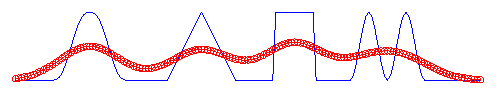
\includegraphics[width=0.5\textwidth]{conver/first}}
	\subfloat[схема Lax"--~Wendroff]{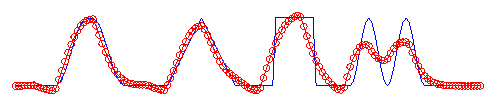
\includegraphics[width=0.5\textwidth]{conver/lw}}\\
	\subfloat[схема Beam"--~Warming]{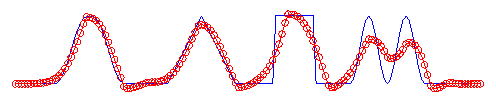
\includegraphics[width=0.5\textwidth]{conver/bw}}
	\subfloat[схема Fromm]{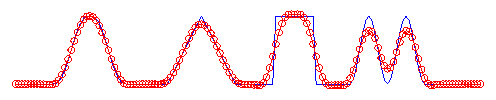
\includegraphics[width=0.5\textwidth]{conver/fromm}}\\
	\subfloat[minmod ограничитель]{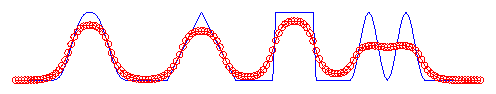
\includegraphics[width=0.5\textwidth]{conver/minmod}}
	\subfloat[van Albada ограничитель]{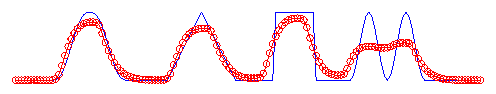
\includegraphics[width=0.5\textwidth]{conver/vanalbada}}\\
	\subfloat[Koren ограничитель]{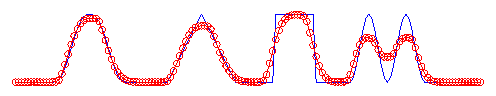
\includegraphics[width=0.5\textwidth]{conver/koren}}
	\subfloat[van Leer ограничитель]{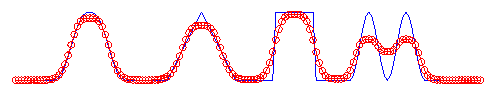
\includegraphics[width=0.5\textwidth]{conver/vanleer}}\\
	\subfloat[superbee ограничитель]{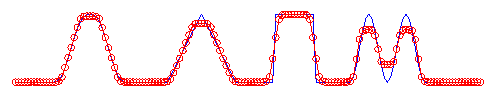
\includegraphics[width=0.5\textwidth]{conver/superbee}}
	\subfloat[MC ограничитель]{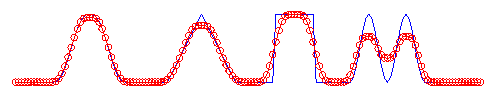
\includegraphics[width=0.5\textwidth]{conver/mc}}\\
	\subfloat[wide superbee ограничитель]{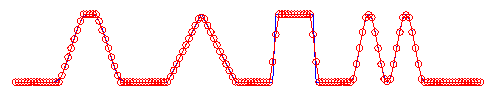
\includegraphics[width=0.5\textwidth]{conver/superbee_g}}
	\subfloat[wide third ограничитель]{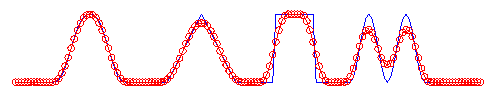
\includegraphics[width=0.5\textwidth]{conver/third_g}}\\
	\centering\subfloat[схема RK3+Koren]{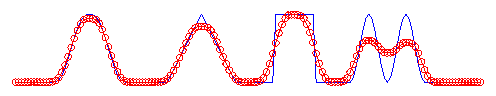
\includegraphics[width=0.5\textwidth]{conver/runge}}
	\caption{Поведение различных схем на различных решениях при числе Куранта \(\gamma=0.5\).}\label{fig:conver}
\end{figure}

Простейшая задача для сравнения ограничителей "--- это одномерная задача переноса с фиксированной скоростью без граничных условий.
На рис.~\ref{fig:conver} представлено поведение всех заявленных ограничителей при числе Куранта \(\gamma=0.5\) слева направо:
на гладком решении, с разрывом производной, разрывом самой функции и для быстро осциллирующего решения.

Сразу видно, что схема первого порядка даёт неудовлетворительные результаты, поскольку ``размазывает'' форму всех импульсов,
поэтому рекомендуется не использовать её для прецизионных расчётов.
Классические схемы (особенно \textit{Fromm}) дают неплохие результаты, однако отсутствие условия TVD влечёт за собой паразитические осцилляции,
в частности, нарушается условие неотрицательности, что особенно важно при решении кинетического уравнения,
поэтому их также стоит непригодными для использования. Отметим, что \textit{Fromm} ввиду своей симметричности лишён фазового сдвига
по сравнению с запаздывающим решением \textit{Lax"--~Wendroff} и опережающим \textit{Beam"--~Warming}.

Наихудшим среди TVD ограничителей второго порядка точности, как и ожидалось, стал \textit{minmod}.
\textit{Van Albada} также плох из-за сильной несимметричности по отношению ко знаку производной функции.
Аналогичные проблемы c ассиметричностью испытывает \textit{Koren}, который приспособлен для схемы Рунге-Кутты (формулы \ref{eq:rk1}--\ref{eq:rk2}).

Лучше всего гладкие решения аппроксимирует \textit{MC}, \textit{van Leer} и \textit{wide third} ограничители,
поскольку они (это относится и к схеме \textit{Fromm}) имеют одинаковое значение производной \(\varphi'(1)\).
Отличия обуславливаются различным поведением при больших градиентах.
Видно, что \textit{wide third} лучше сходится к экстремумам функции.
Напомним, что, кроме прочего, \textit{wide third} имеет третий порядок сходимости при любых \(\gamma\) в отличие от конкурентов
(значение \(\gamma=0.5\) выбрано специально для сравнения схем третьего порядка).

В сходимости к разрывным и быстро осциллирующим решениям с большим перевесом первенствует \textit{wide superbee},
который также по всем показателям обошел своего классического коллегу \textit{superbee}.

Для численного сравнения ограничителей использовалась октаэдрическая норма:
\begin{equation}\label{eq:norm}
	D(M) = \|f-v\| = \frac1{M}\sum_{i=1}^{M}|f_i-v_i| = \mathcal{O}(h^q),
\end{equation}
где \(v_i\) "--- точное решение, \(h\) "--- сеточный шаг, \(q\) "--- порядок сходимости, \(M\) "--- общее число ячеек.
На гладких решениях порядок сходимости при условии сходимости совпадает с порядком аппроксимации согласно теореме Лакса"--~Рябенького.
В противном случае на сегодняшний день теоретический анализ затруднителен, поэтому будем использовать экспериментальные значения.
В табл.~\ref{tab:q_value} представлены соответствующие значения порядков сходимости исследуемых схем при различных числах Куранта
для решений с разрывами значения и первых трёх производных. Они вычислялись по простой формуле
\[ q = \log_2\frac{D(M)}{D(2M)} \]
для следующих функций:
\begin{alignat*}{2}
	 g_0(x) &= 1,\quad &|x| < 1, \\
	 g_1(x) &= 1-|x|,\quad &|x| < 1, \\
	 g_2(x) &= 1-3|x|^2+2|x|^3,\quad &|x| < 1, \\
	 g_3(x) &= 1-10|x|^3+15|x|^4-6|x|^5,&\quad |x| < 1. 
\end{alignat*}
Аналогичное сравнение широкого класса численных схем можно найти в \cite{Safronov2010}.

Схема \textit{first} везде имеет первый порядок сходимости, кроме разрывных решений,
где значение \(q=0.5\) объясняется схемной вязкостью (получается в дифференциальном приближении).
Остальные схемы отчетливо проявили свой порядок на гладком решении,
поэтому в таких случаях предпочтение стоит отдать схемам третьего порядка \textit{wide third} и \textit{RK3+Koren},
однако последняя требует б\textit{о}льшего объёма вычислений.

Что касается разрывных решений, то максимальный порядок (\(q=1\)) продемострировали \textit{superbee} и \textit{wide superbee}.
Выделение класса схем с единичным порядком "--- сложная задача, но, по-видимому,
\textit{superbee} схемы представляют собой наилучшее сочетание со вторым порядком аппроксимации.

\ctable[
	caption = Порядки сходимости исследуемых схем,
	label = tab:q_value,
]{|l|c|c|c|c||c|c|c|c|}{
	\tnote{Все экспериментальные значения порядков сходимости получены при сравнении невязок для одинаковых сеток
		с числом ячеек \(N\sim10^3\), приходящихся на ненулевые значения начальной функции.
		При дальнейшем увеличении объёма расчетной сетки порядок сходимости практически не меняется, однако
		в этом случае наблюдается исключение, поскольку значение \(q(N)\) неравномерно убывает с умельчением расчётной сетки
		от \(q(16)=1.76\) до \(q(16\cdot10^3)=0.55\) и далее.
		Это связано с особенностями начальной функции \(g_1(x)\), у которой везде, где \(\exists g''_1\), \(g''_1=0\),
		а это соответствует точке \(\theta=1\), колебания возле которой приводят к значительной потере сходимости.
		Дабы не умалять достоинств \textit{wide superbee} отметим, что он вплоть до сеток с \(N\simeq2\cdot10^3\) обладает наименьшей абсолютной невязкой.}
}{
	\hline
	\multirow{2}{*}{Лимитер} & \multicolumn{4}{c||}{\(\gamma=0.5\)} & \multicolumn{4}{c|}{\(\gamma=0.9\)} \\ \cline{2-9}
	& \(\nexists f\) & \(\nexists f'\) & \(\nexists f''\) & \(\nexists f'''\) 
	& \(\nexists f\) & \(\nexists f'\) & \(\nexists f''\) & \(\nexists f'''\) \\ \hline
	first order				& 0.500 & 1.000 & 0.991 & 0.983 & 0.500 & 1.000 & 0.998 & 0.997 \\ \hline
	Lax"--~Wendroff			& 0.674 & 1.280 & 1.956 & 1.993 & 0.582 & 1.233 & 1.964 & 1.999 \\ \hline
	Beam"--~Warming			& 0.674 & 1.280 & 1.956 & 1.993 & 0.668 & 1.291 & 1.986 & 1.999 \\ \hline
	Fromm					& 0.765 & 1.505 & \color{magenta}2.520 & \color{magenta}2.950 & 0.619 & 1.282 & 1.978 & 1.998 \\ \hline
	minmod					& 0.662 & 1.325 & 1.925 & 1.982 & 0.658 & 1.322 & 1.940 & 1.990 \\ \hline
	van Albada				& 0.675 & 1.323 & 1.954 & 1.999 & 0.670 & 1.307 & 1.967 & 1.999 \\ \hline
	van Leer				& 0.747 & 1.486 & \color{magenta}2.212 & \color{magenta}2.933 & 0.707 & 1.414 & 2.033 & 2.002 \\ \hline
	Koren					& 0.667 & 1.333 & 1.964 & 2.000 & 0.660 & 1.305 & 1.967 & 2.000 \\ \hline
	MC						& 0.752 & 1.534 & \color{magenta}2.424 & \color{magenta}2.931 & 0.691 & 1.397 & 1.991 & 2.000 \\ \hline
	superbee				& \color{olive}1.000 & 1.519 & 1.933 & 2.000 & \color{olive}0.997 & 1.500 & 1.961 & 2.000 \\ \hline
	wide superbee			& \color{olive}1.000 & 1.694 & 1.933 & 2.000 & \color{olive}1.000 & \(\sim\)1.7\tmark & 1.959 & 2.000 \\ \hline
\color{magenta}	wide third	& 0.749 & 1.508 & \color{magenta}2.597 & \color{magenta}2.918 & 0.747 & 1.534 & \color{magenta}2.530 & \color{magenta}2.947 \\ \hline
\color{magenta}	RK3+Koren	& 0.753 & 1.541 & \color{magenta}2.445 & \color{magenta}2.905 & 0.751 & 1.511 & \color{magenta}2.428 & \color{magenta}2.899 \\ \hline
}

Кроме порядка сходимости основной интерес представляет также абсолютное значение невязки.
На рис.~\ref{fig:residual} показана зависимость невязки от количества ячеек \(N\), приходящихся на ненулевое значение \(f(0,x)\).
Приведены для краткости только ограничители \textit{superbee} и третьего порядка в сравнении с классическими схемами.
На гладких функциях, как и предполагалось, наименьшую невязку на мелких сетках показал \textit{wide third},
однако на грубых сетках благодаря большим антидиффузионным потокам отличный результат показывает \textit{wide superbee}.
На разрывных решениях у всех схем невязка уменьшается практически линейно.

\begin{figure}[h]
		\subfloat[гладкая функция, \(\gamma=0.5\)]{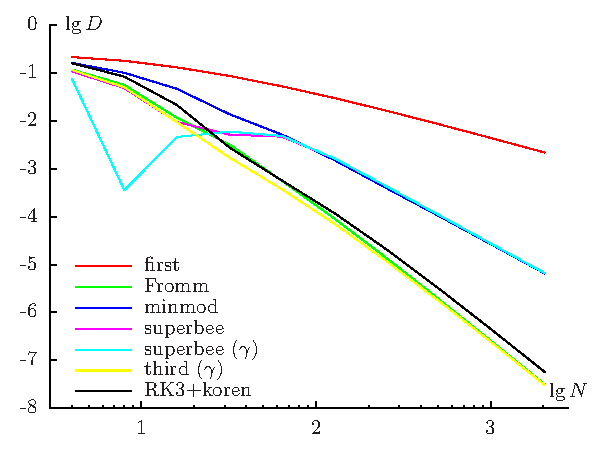
\includegraphics[width=0.5\textwidth]{residual/05_3dis.pdf}}
		\subfloat[гладкая функция, \(\gamma=0.9\)]{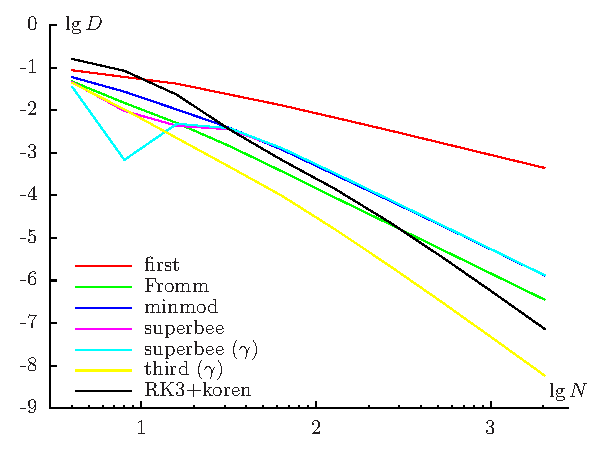
\includegraphics[width=0.5\textwidth]{residual/09_3dis.pdf}}\\
		\subfloat[разрывная функция, \(\gamma=0.5\)]{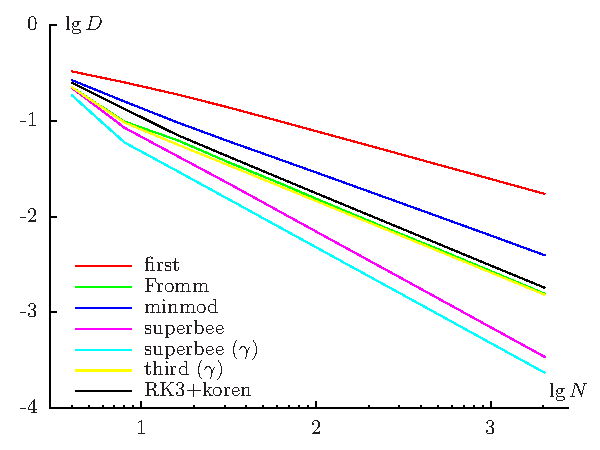
\includegraphics[width=0.5\textwidth]{residual/05_0dis.pdf}}
		\subfloat[разрывная функция, \(\gamma=0.9\)]{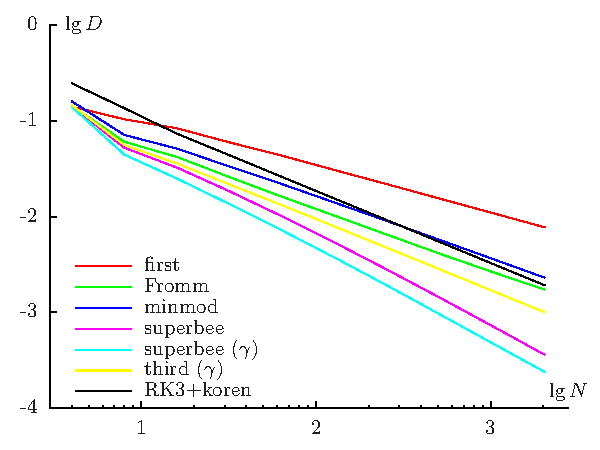
\includegraphics[width=0.5\textwidth]{residual/09_0dis.pdf}}
	\caption{Зависимость невязки от мелкости сетки.}\label{fig:residual}
\end{figure}

\section*{\centering{Заключение}}
В результате исследования можно выделить две наилучших схемы.
Для решения нестационарных задач с большими градиентами (например, в случае ударных волн)
и при использовании грубых сеток для быстрых расчётов рекомендуется использовать \textit{wide superbee}.
Наилучшую сходимость к гладким функциям (что обычно характерно для стационарных распределений) показал \textit{wide third},
что определяет его применимость для прецизионных вычислений.

\centering{\bibliographystyle{abbrv}}
\bibliography{lim,lim_rus}

\end{document}
